\block{}{
  \begin{tikzfigure}[First iteration of Phase 1]
    %\centering
    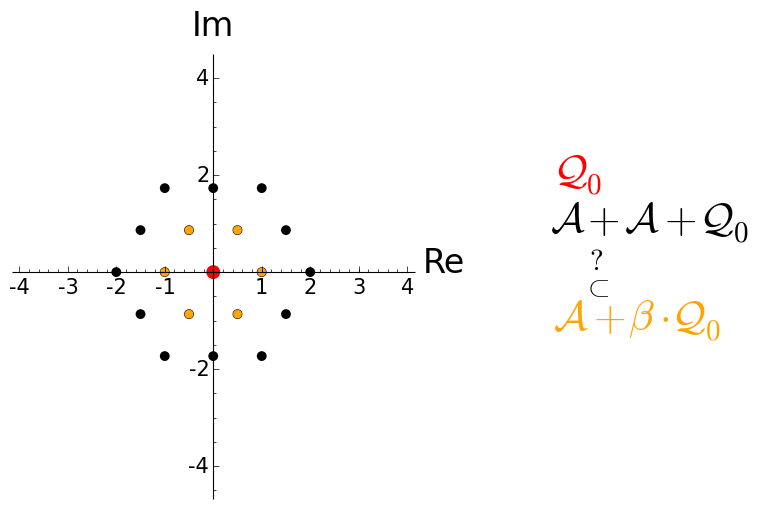
\includegraphics[width=0.2\textwidth]{img/phase1_image_3a.png}
    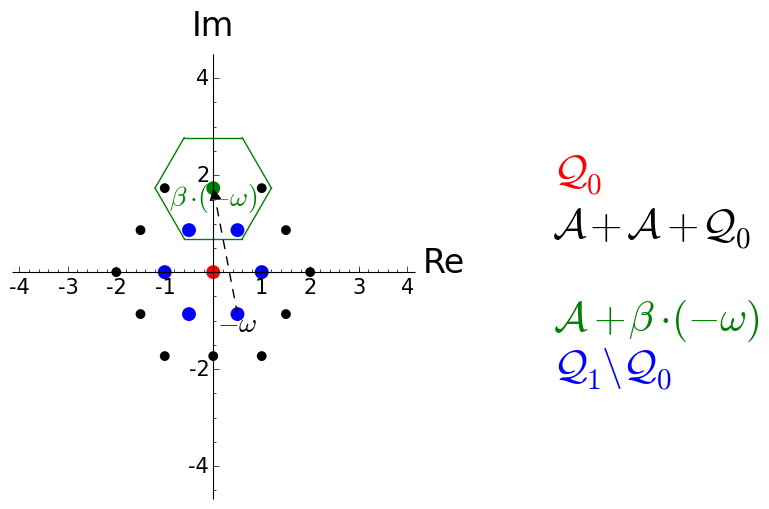
\includegraphics[width=0.2\textwidth]{img/phase1_image_4.png}
\end{tikzfigure}
}

\note[targetoffsetx=-.2\colwidth,targetoffsety=0\colwidth,innersep=0.5cm,angle=-135,connection, width=15cm]{\rule{15cm}{0cm} Eisenstein base $$\beta = \omega -1\,,\omega=-\frac{1}{2} + \frac{\imath \sqrt{3}}{2}\,.$$

The minimal polynomial $$m_\beta(x)=x^2+3x+3\,.$$

Alphabet $$\mathcal{A} =\{0, 1, -1, \omega, -\omega, -\omega - 1, \omega + 1\}$$}
